Data for this project was collected by the US. Army Corps of Engineers (USACE) Engineer Research and Development Center (ERDC) during October 2015 at the Field Research Facility (FRF) in Duck, NC on the Outerbanks shown in Figure~\ref{FRFmap}.\footnote{The data can be accessed online at http://chlthredds.erdc.dren.mil/thredds/catalog/frf/projects/bathyduck/catalog.html} The data was collected via the BathyDuck project conducted by the Coastal and Hydraulic Laboratory (CHL). Data of interest includes wave height (\textit{H}), wave number (\textit{k}), wave period (\textit{T}), and bathymetry (\textit{h}) measurements. These data combine information collected through a Nortek Acoustic Wave and Current (AWAC) Profiler, a Light Amphibious Resupply Cargo (LARC-5) vessel, a Coastal Research Amphibious Buggy (CRAB), and Argus Beach Monitoring systems. The LARC-5 and CRAB vessels are shown below in Figure ~\ref{crablarc}.

\begin{figure}[h]
\centering
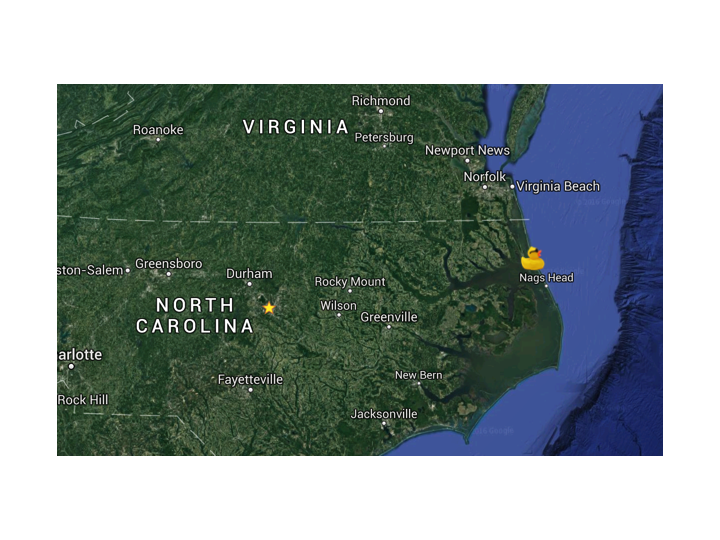
\includegraphics[width=.48\linewidth]{img/FRF_map.png}
\caption{The location of the U.S. Army Corps of Engineers Field Research Facility in Duck, NC.}
\label{FRFmap}
\end{figure}

\begin{figure}[h]
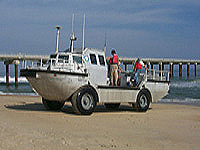
\includegraphics[width=.48\linewidth]{img/LARC.jpg}\hfill
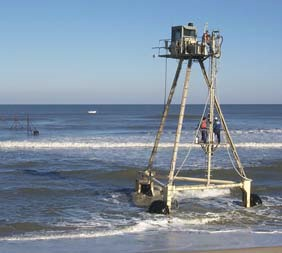
\includegraphics[width=.48\linewidth]{img/CRAB2.JPG}
\caption{The LARC (left) and CRAB (right) instruments are used to measure near coastal bathymetry. Image source: http://www.frf.usace.army.mil/aboutUS/equipment.shtml}
\label{crablarc}
\end{figure}

The following sections discuss in more detail the observations and how they were used. Please note that in physical space, the boundary point used for the 1-dimensional problem is located 1150 m offshore. For numerical simplicity, all observations are transformed such that $\textit{x}$ = 0 m corresponds to the offshore boundary point and $\textit{x}$ = 1150 m is the shoreline. 

